\documentclass[12pt, a4paper]{report}
\usepackage[utf8]{inputenc}
\usepackage[T1]{fontenc}
\usepackage[french]{babel}
\usepackage{geometry}
\usepackage{graphicx}
\usepackage{listings}
\usepackage{xcolor}
\usepackage{fancyhdr}
\usepackage{titlesec}
\usepackage{booktabs}
\usepackage{array}
\usepackage{hyperref}
\usepackage{setspace}
\usepackage{tcolorbox}
\usepackage{caption}

\usepackage{float}

\geometry{top=2.5cm, bottom=2.5cm, left=3cm, right=2.5cm}

% Couleurs
\definecolor{codeblue}{RGB}{0, 102, 204}
\definecolor{codegray}{RGB}{245, 245, 245}
\definecolor{codecomment}{RGB}{106, 153, 85}
\definecolor{codestring}{RGB}{206, 145, 120}
\definecolor{codekeyword}{RGB}{86, 156, 214}
\definecolor{titlecolor}{RGB}{0, 70, 127}
\definecolor{sectioncolor}{RGB}{0, 102, 204}

% Style des listings SQL
\lstdefinestyle{sqlstyle}{
    backgroundcolor=\color{codegray},
    commentstyle=\color{codecomment}\itshape,
    keywordstyle=\color{codekeyword}\bfseries,
    stringstyle=\color{codestring},
    basicstyle=\ttfamily\small,
    breakatwhitespace=false,
    breaklines=true,
    keepspaces=true,
    numbers=left,
    numbersep=8pt,
    numberstyle=\tiny\color{gray},
    showspaces=false,
    showstringspaces=false,
    showtabs=false,
    tabsize=4,
    frame=single,
    rulecolor=\color{codeblue},
    morekeywords={
        CREATE, TABLE, OR, REPLACE, PROCEDURE, IS, BEGIN, END,
        INSERT, INTO, VALUES, UPDATE, SET, WHERE, SELECT, FROM,
        DECLARE, CURSOR, FOR, LOOP, IF, THEN, ELSIF, ELSE,
        EXCEPTION, WHEN, OTHERS, ROLLBACK, COMMIT, RETURN,
        SEQUENCE, START, WITH, INCREMENT, BY, REFERENCES,
        CONSTRAINT, PRIMARY, KEY, DEFAULT, NULL, SYSDATE,
        DBMS_OUTPUT, PUT_LINE, SQLERRM, NEXTVAL, COUNT,
        NUMBER, VARCHAR2, DATE, IN, OUT, TYPE, RPAD,
        GROUP, ACCEPT, PROMPT, COLUMN, NEW_VALUE, NOPRINT,
        CASE, DUAL, SQL, NOTFOUND, AND, NOT
    }
}
\lstset{style=sqlstyle}

% En-tête et pied de page
\pagestyle{fancy}
\fancyhf{}
\fancyhead[L]{\textcolor{sectioncolor}{\small Projet de Base de Données 2}}
\fancyhead[R]{\textcolor{sectioncolor}{\small Université Nazi Boni}}
\fancyfoot[C]{\thepage}
\renewcommand{\headrulewidth}{0.4pt}
\renewcommand{\footrulewidth}{0.4pt}

% Style des titres
\titleformat{\chapter}[display]
  {\normalfont\huge\bfseries\color{titlecolor}}
  {\chaptertitlename\ \thechapter}{20pt}{\Huge}
\titleformat{\section}
  {\normalfont\Large\bfseries\color{sectioncolor}}
  {\thesection}{1em}{}
\titleformat{\subsection}
  {\normalfont\large\bfseries\color{sectioncolor!80}}
  {\thesubsection}{1em}{}

\hypersetup{
    colorlinks=true,
    linkcolor=sectioncolor,
    urlcolor=sectioncolor,
}

\begin{document}

% ============================================================
% PAGE DE GARDE
% ============================================================
\begin{titlepage}
    \thispagestyle{empty}

    % Bandeau bleu en haut
    \noindent
    \begin{tcolorbox}[colback=titlecolor, colframe=titlecolor,
                      width=\textwidth, halign=center]
        \centering
        \textcolor{white}{\large \textbf{BURKINA FASO}}\\[0.2cm]
        \textcolor{white}{\normalsize \textit{La Patrie ou la Mort Nous vaincrons}}
    \end{tcolorbox}

    \vspace{1cm}

    % Logos + textes institutions
    \noindent
    \begin{minipage}[t]{0.45\textwidth}
        \centering
        % Logo Burkina Faso ici
     
        
\includegraphics[width=2.2cm]{logo_bf.png}\\[6pt]
        \small
        \textsf{Ministère de l'Enseignement}\\
        \textsf{Supérieur, de la Recherche}\\
        \textsf{et de l'Innovation}
    \end{minipage}
    \hfill
    \begin{minipage}[t]{0.45\textwidth}
        \centering
        % Logo UNB ici
        
\includegraphics[width=2.2cm]{logo_unb.png}\\[6pt]        
        \small
        \textsf{Université Nazi Boni}\\
        \textsf{UFR Sciences Exactes et Appliquées}\\
        \textsf{Licence Statistiques et Informatique}
    \end{minipage}

    \vspace{1cm}
    \rule{\linewidth}{0.8pt}
    \vspace{0.5cm}

    \begin{center}
        {\Large \textbf{RAPPORT DE PROJET}}\\[0.3cm]
        {\normalsize \textit{Sur le thème :}}
    \end{center}

    \vspace{0.5cm}

    \begin{tcolorbox}[colback=sectioncolor!15, colframe=sectioncolor,
                      width=\textwidth, halign=center]
        \centering
        \textcolor{sectioncolor}{\large \textbf{Gestion d'une Bibliothèque Universitaire}}\\[0.3cm]
        \textcolor{sectioncolor}{\large \textbf{avec Procédures PL/SQL}}\\[0.3cm]
        \textcolor{sectioncolor}{\normalsize \textbf{Oracle SQL*Plus --- Base de Données 2}}
    \end{tcolorbox}

    \vspace{0.8cm}

    \begin{center}
        \textit{Présenté par les membres du groupe :}\\[0.5cm]
        {\large \textbf{SAKO Biton F.B Chérif}}\\[0.2cm]
        {\large \textbf{BAYARA Orianne.E.A}}\\[0.2cm]
        {\large \textbf{ILBOUDO B.G Bryand}}\\[0.3cm]
        {\small Étudiants en Licence 2 --- Statistiques et Informatique}
    \end{center}

    \vfill

    \rule{\linewidth}{0.8pt}\\[0.3cm]
    \noindent
    \begin{minipage}[t]{0.5\textwidth}
        \textbf{Chargé du cours :}\\[0.2cm]
        Dr Go Issa TRAORE\\
        \textit{Année académique 2025--2026}
    \end{minipage}
    \hfill
    \begin{minipage}[t]{0.4\textwidth}
        \raggedleft
        \textbf{Date de remise :}\\[0.2cm]
        04 Mai 2026
    \end{minipage}

\end{titlepage}

% ============================================================
% TABLE DES MATIÈRES
% ============================================================
\tableofcontents
\newpage

% ============================================================
% INTRODUCTION
% ============================================================
\chapter{Introduction}

Dans un monde en perpétuel évolution où les données occupent une place centrale, la maîtrise des outils (tel que SQL*Plus d'Oracle) de gestion, d'exploitation et d'analyse des bases de données constitue une compétence fondamentale pour tout professionnel de l'informatique et de la data.
Pour ces derniers, la maîtrise de SQL*Plus représente un avantage considérable.
Elle permet un accès direct aux données sans intermédiaire, une automatisation
des pipelines de traitement et une performance optimale sur de grands volumes de données.
C'est dans cette perspective que s'inscrit ce projet de base de données 2,
réalisé dans le cadre de notre formation en Licence 2 Statistiques et
Informatique à l'Université Nazi Boni. Il nous a été confié par notre
enseignant Dr Go Issa TRAORE et porte sur la \textbf{Gestion d'une
Bibliothèque Universitaire avec des Procédures PL/SQL}.
Ce rapport est organisé comme suit : nous présentons d'abord la modélisation
des données, suivie des scripts de création des tables. Nous détaillons ensuite
les procédures stockées développées ainsi que le menu interactif conçu.
Enfin, nous présentons les tests réalisés et les résultats obtenus.

% ============================================================
% MODÉLISATION
% ============================================================
\chapter{Modélisation des données}

\section{Entités}
Le système repose sur trois entités principales :

\begin{center}
	\begin{tabular}{|>{\bfseries}l|l|}
		\hline
		\textbf{Entité} & \textbf{Attributs} \\
		\hline
		Livre & liv\_id, titre, auteur, disponibilite, statut, motif \\
		\hline
		Abonné & abon\_id, nom, prenom, statut, motif \\
		\hline
		Emprunt & emprunt\_id, liv\_id, abon\_id, date\_emprunt, date\_retour \\
		\hline
	\end{tabular}
\end{center}

\section{Choix de conception}
Plusieurs décisions ont guidé la conception du système.

Chaque exemplaire d'un livre possède son propre identifiant unique,
généré automatiquement par une séquence (\texttt{LIV1}, \texttt{LIV2}, ...). En effet, pour la bonne gestion de la bibliothèque, nous avons consideé deux exemplaires du même ouvrage comme étant deux objets distincts.
Chaque abonné (étudiant comme enseignant) est reconnu par un identifiant qui lui est propre, généré automatiquement également par une séquence (\texttt{ABN1}, \texttt{ABN2}, ...). 
Dans les tables \textbf{livre} et \textbf{abonne}, deux nouveaux attributs ont été ajoutés à savoir \textbf{statut et motif}. Pour la table \textbf{livre}, \textbf{statut} est par défaut "actif" à chaque insertion d'un nouveau livre et passe à "inactif" si le livre est supprimé de la base de données. Concernant l'attribut \textbf{motif}, il prend pour valeur le motif de la suppression du livre.
Pour la table \textbf{abonne}, \textbf{statut} est par défaut "actif" également à chaque insertion d'un nouveau abonné et passe à "inactif" s'il se désabonne de la bibliothèque. Quant à \textbf{motif}, il prend ici aussi le motif du désabonnement d'un abonné.
Au niveau de la table \textbf{emprunt}, nous avons inséré un nouvel attribut qui est \textbf{date\_retour}. Cet attribut est initialisé à \textbf{null} et est mis à jour à la date du retour du livre emprunté.
Plutôt que de supprimer physiquement les données d'un abonné désabonné ou
d'un livre retiré, on adopte une \textbf{suppression logique} : le champ
\texttt{statut} passe à \texttt{'Inactif'} et le champ \texttt{motif}
enregistre la raison, garantissant ainsi la traçabilité des données. 

\subsection*{Procédures supplémentaires (4.6 à 4.10)}

Le projet demandait cinq procédures de base. Nous en avons ajouté cinq autres
pour rendre le système réellement utilisable :

\begin{itemize}
	\item \textbf{4.6 — \texttt{affichage\_emprunt} :} permet de consulter
	les emprunts en cours et l'historique des sorties, informations essentielles
	pour le bibliothécaire.
	
	\item \textbf{4.7 — \texttt{affichage\_abonne} :} permet de vérifier
	rapidement si un étudiant est inscrit et de connaître son statut.
	
	\item \textbf{4.8 — \texttt{supprimer\_livre} :} permet de retirer un
	livre perdu ou abîmé du registre, sans le supprimer physiquement, en
	enregistrant le motif,tout en bloquant la suppression si le livre est
	en emprunt.
	
	\item \textbf{4.9 — \texttt{desabonne} :} permet de désactiver
	un abonné qui quitte l'université ou si son abonnement prend fin, tout en bloquant le désabonnement si
	un emprunt est encore en cours.
	
	\item \textbf{4.10 — \texttt{reabonnement} :} elle permet de réactiver un abonné précédemment désabonné.
\end{itemize}

\subsection*{ Création de séquences}
Nous avons créé trois séquences pour générer des identifiants automatiquement. Il s'agit de:  

\begin{itemize}
	

	\item \textbf{seq\_livre}, qui permet de générer automatiquement les identifiants des livres
	sous la forme \texttt{LIV1}, \texttt{LIV2}, \texttt{LIV3}... à chaque ajout.
	
	\item \textbf{seq\_abonne}, qui permet de générer automatiquement les identifiants des abonnés
	sous la forme \texttt{ABN1}, \texttt{ABN2}, \texttt{ABN3}... à chaque ajout.
	
	\item \textbf{seq\_emprunt}, génère automatiquement les identifiants des emprunts
	sous la forme \texttt{1}, \texttt{2}, \texttt{3}... à chaque nouvel emprunt enregistré.
	
\end{itemize}
% ============================================================
% SCRIPTS DE CRÉATION DES TABLES
% ============================================================
\chapter{Scripts de création des tables}

\section{Table LIVRE}
\begin{lstlisting}[language=SQL, caption=Création de la table Livre]
	create table livre (
	liv_id        varchar2(10)  constraint pk1 primary key,
	titre         varchar2(100),
	auteur        varchar2(200),
	disponibilite varchar2(5)   default null,
	statut        varchar2(10)  default 'Actif',
	motif         varchar2(200) default null);
\end{lstlisting}

\section{Table ABONNE}
\begin{lstlisting}[language=SQL, caption=Création de la table Abonné]
	create table abonne (
	abon_id varchar2(20)  constraint pk2 primary key,
	nom     varchar2(50),
	prenom  varchar2(20),
	statut  varchar2(10)  default 'Actif',
	motif   varchar2(200) default null);
\end{lstlisting}

\section{Table EMPRUNT}
\begin{lstlisting}[language=SQL, caption=Création de la table Emprunt]
	create table emprunt (
	emprunt_id   number        constraint pk3 primary key,
	liv_id       varchar2(10)  references livre,
	abon_id      varchar2(20)  references abonne,
	date_emprunt date          default null,
	date_retour  date          default null
	);
\end{lstlisting}

\section{Séquences}
\begin{lstlisting}[language=SQL, caption=Création des séquences]
	create sequence seq_livre   start with 1 increment by 1;
	create sequence seq_emprunt start with 1 increment by 1;
\end{lstlisting}

% ============================================================
% SCRIPTS DES PROCÉDURES
% ============================================================
\chapter{Scripts des procédures}

\section{Procédure : Ajout d'un livre}
\begin{lstlisting}[language=SQL, caption=Procédure ajout\_livre]
	create or replace procedure ajout_livre(
	title      in livre.titre%type,
	auteur_liv in livre.auteur%type)
	is
	v_id livre.liv_id%type;
	begin
	select 'LIV' || seq_livre.nextval into v_id from dual;
	insert into livre values(v_id, title, auteur_liv, 'Oui', 'Actif', null);
	commit;
	dbms_output.put_line('Le livre ' || v_id || ' ' || title
	|| ' a ete ajoute avec succes');
	exception
	when others then
	dbms_output.put_line('Erreur!! ' || SQLERRM);
	rollback;
	end ajout_livre;
	/
\end{lstlisting}

\section{Procédure : Ajout d'un abonné}
\begin{lstlisting}[language=SQL, caption=Procédure ajout\_abonne]
	create or replace procedure ajout_abonne(
	id       in abonne.abon_id%type,
	nom_a    in abonne.nom%type,
	prenom_a in abonne.prenom%type)
	is
	v_count number;
	begin
	select count(*) into v_count from abonne where abon_id = id;
	if v_count > 0 then
	dbms_output.put_line('Erreur!! L''INE ' || id
	|| ' existe deja dans la base de donnees.');
	dbms_output.put_line(
	'Impossible d''enregistrer deux etudiants avec le meme INE.');
	return;
	end if;
	insert into abonne values(id, nom_a, prenom_a, 'Actif', null);
	commit;
	dbms_output.put_line('L''abonne ' || id || ' ' || nom_a
	|| ' ' || prenom_a || ' a ete ajoute avec succes');
	exception
	when others then
	dbms_output.put_line('Erreur!! ' || SQLERRM);
	rollback;
	end ajout_abonne;
	/
\end{lstlisting}

\section{Procédure : Emprunt d'un livre}
\begin{lstlisting}[language=SQL, caption=Procédure emprunt\_livre]
	create or replace procedure emprunt_livre(
	id_liv    in livre.liv_id%type,
	id_abonne in abonne.abon_id%type)
	is
	v_dispo         livre.disponibilite%type;
	v_statut_liv    livre.statut%type;
	v_statut_abon   abonne.statut%type;
	v_count_liv     number;
	v_count_abon    number;
	v_count_emprunt number;
	begin
	select count(*) into v_count_liv from livre where liv_id = id_liv;
	select count(*) into v_count_abon from abonne where abon_id = id_abonne;
	
	if v_count_liv = 0 then
	dbms_output.put_line(
	'Erreur!! Ce livre n''existe pas dans la base de donnees.');
	return;
	end if;
	if v_count_abon = 0 then
	dbms_output.put_line(
	'Erreur!! Cet abonne n''existe pas dans la base de donnees.');
	return;
	end if;
	
	select statut into v_statut_liv from livre where liv_id = id_liv;
	if v_statut_liv = 'Inactif' then
	dbms_output.put_line(
	'Erreur!! Ce livre a ete retire de la bibliotheque.');
	return;
	end if;
	
	select statut into v_statut_abon from abonne where abon_id = id_abonne;
	if v_statut_abon = 'Inactif' then
	dbms_output.put_line(
	'Erreur!! Cet abonne est desabonne de la bibliotheque.');
	return;
	end if;
	
	select count(*) into v_count_emprunt
	from emprunt where abon_id = id_abonne and date_retour is null;
	if v_count_emprunt > 0 then
	dbms_output.put_line(
	'Erreur!! Cet abonne a deja un livre en cours d''emprunt.');
	dbms_output.put_line(
	'Il doit rendre le livre avant d''en emprunter un autre.');
	return;
	end if;
	
	select disponibilite into v_dispo from livre where liv_id = id_liv;
	if v_dispo = 'Oui' then
	insert into emprunt(emprunt_id, liv_id, abon_id, date_emprunt)
	values(seq_emprunt.nextval, id_liv, id_abonne, sysdate);
	update livre set disponibilite = 'Non' where liv_id = id_liv;
	commit;
	dbms_output.put_line('L''emprunt a ete effectue avec succes');
	else
	dbms_output.put_line(
	'Ce livre n''est plus disponible dans la bibliotheque');
	end if;
	exception
	when others then
	dbms_output.put_line('Erreur!! ' || SQLERRM);
	rollback;
	end emprunt_livre;
	/
\end{lstlisting}

\section{Procédure : Retour d'un livre}
\begin{lstlisting}[language=SQL, caption=Procédure retour\_livre]
	create or replace procedure retour_livre(
	id_liv    in livre.liv_id%type,
	id_abonne in abonne.abon_id%type)
	is
	v_count_liv  number;
	v_count_abon number;
	begin
	select count(*) into v_count_liv from livre where liv_id = id_liv;
	select count(*) into v_count_abon from abonne where abon_id = id_abonne;
	
	if v_count_liv = 0 then
	dbms_output.put_line(
	'Erreur!! Ce livre n''existe pas dans la base de donnees.');
	return;
	end if;
	if v_count_abon = 0 then
	dbms_output.put_line(
	'Erreur!! Cet abonne n''existe pas dans la base de donnees.');
	return;
	end if;
	
	update emprunt set date_retour = sysdate
	where liv_id = id_liv and abon_id = id_abonne and date_retour is null;
	
	if SQL%NOTFOUND then
	dbms_output.put_line(
	'Aucun emprunt en cours trouve pour ce livre et cet abonne.');
	return;
	end if;
	
	update livre set disponibilite = 'Oui' where liv_id = id_liv;
	commit;
	dbms_output.put_line('Le retour du livre a ete effectue avec succes');
	exception
	when others then
	dbms_output.put_line('Erreur!! ' || SQLERRM);
	rollback;
	end retour_livre;
	/
\end{lstlisting}

\section{Procédure : Affichage des livres disponibles}
\begin{lstlisting}[language=SQL, caption=Procédure affichage\_livre]
	create or replace procedure affichage_livre
	is
	cursor info is
	select titre, auteur, count(*) as nb_exemplaires
	from livre
	where disponibilite = 'Oui' and statut = 'Actif'
	group by titre, auteur;
	v_count number := 0;
	begin
	dbms_output.put_line(
	'================================================================');
	dbms_output.put_line(
	'  TITRE                | AUTEUR              | DISPONIBILITE    ');
	dbms_output.put_line(
	'================================================================');
	for i in info loop
	v_count := v_count + 1;
	dbms_output.put_line(
	'  ' || rpad(i.titre, 20) || ' | '
	|| rpad(i.auteur, 19) || ' | '
	|| i.nb_exemplaires || ' exemplaire(s)');
	end loop;
	dbms_output.put_line(
	'================================================================');
	if v_count = 0 then
	dbms_output.put_line('  Aucun livre disponible.');
	dbms_output.put_line(
	'================================================================');
	end if;
	exception
	when others then
	dbms_output.put_line('Erreur!! ' || SQLERRM);
	end affichage_livre;
	/
\end{lstlisting}

\section{Procédure : Affichage des emprunts}
\begin{lstlisting}[language=SQL, caption=Procédure affichage\_emprunt]
	create or replace procedure affichage_emprunt
	is
	cursor info is
	select a.nom, a.prenom, l.titre,
	e.date_emprunt, e.date_retour
	from emprunt e
	join abonne a on e.abon_id = a.abon_id
	join livre  l on e.liv_id  = l.liv_id
	order by e.date_emprunt;
	v_count number := 0;
	begin
	dbms_output.put_line(
	'=================================================================');
	dbms_output.put_line(
	'  ABONNE         | TITRE                | D.EMPRUNT  | D.RETOUR ');
	dbms_output.put_line(
	'=================================================================');
	for i in info loop
	v_count := v_count + 1;
	dbms_output.put_line(
	'  ' || rpad(i.nom || ' ' || i.prenom, 14) || ' | '
	|| rpad(i.titre, 20) || ' | '
	|| to_char(i.date_emprunt, 'DD/MM/YYYY') || ' | '
	|| case
	when i.date_retour is null then 'En cours'
	else to_char(i.date_retour, 'DD/MM/YYYY')
	end);
	end loop;
	dbms_output.put_line(
	'=================================================================');
	if v_count = 0 then
	dbms_output.put_line('  Aucun emprunt enregistre.');
	dbms_output.put_line(
	'=================================================================');
	end if;
	exception
	when others then
	dbms_output.put_line('Erreur!! ' || SQLERRM);
	end affichage_emprunt;
	/
\end{lstlisting}

\section{Procédure : Affichage des abonnés}
\begin{lstlisting}[language=SQL, caption=Procédure affichage\_abonne]
	create or replace procedure affichage_abonne
	is
	cursor info is
	select abon_id, nom, prenom, statut
	from abonne order by nom;
	v_count number := 0;
	begin
	dbms_output.put_line(
	'================================================================');
	dbms_output.put_line(
	'  INE                  | NOM               | PRENOM  | STATUT  ');
	dbms_output.put_line(
	'================================================================');
	for i in info loop
	v_count := v_count + 1;
	dbms_output.put_line(
	'  ' || rpad(i.abon_id, 20) || ' | '
	|| rpad(i.nom, 17)     || ' | '
	|| rpad(i.prenom, 7)   || ' | '
	|| i.statut);
	end loop;
	dbms_output.put_line(
	'================================================================');
	if v_count = 0 then
	dbms_output.put_line('  Aucun abonne enregistre.');
	dbms_output.put_line(
	'================================================================');
	end if;
	exception
	when others then
	dbms_output.put_line('Erreur!! ' || SQLERRM);
	end affichage_abonne;
	/
\end{lstlisting}

\section{Procédure : Retrait d'un livre}
\begin{lstlisting}[language=SQL, caption=Procédure supprimer\_livre]
	create or replace procedure supprimer_livre(
	id      in livre.liv_id%type,
	p_motif in livre.motif%type)
	is
	v_count_liv number;
	v_dispo     livre.disponibilite%type;
	v_statut    livre.statut%type;
	begin
	select count(*) into v_count_liv from livre where liv_id = id;
	if v_count_liv = 0 then
	dbms_output.put_line(
	'Erreur!! Ce livre n''existe pas dans la base de donnees.');
	return;
	end if;
	
	select statut into v_statut from livre where liv_id = id;
	if v_statut = 'Inactif' then
	dbms_output.put_line(
	'Erreur!! Ce livre est deja retire de la bibliotheque.');
	return;
	end if;
	
	select disponibilite into v_dispo from livre where liv_id = id;
	if v_dispo = 'Non' then
	dbms_output.put_line('Erreur!! Ce livre est actuellement emprunte.');
	dbms_output.put_line(
	'Impossible de le retirer tant qu''il n''est pas rendu.');
	return;
	end if;
	
	update livre set statut = 'Inactif', motif = p_motif where liv_id = id;
	commit;
	dbms_output.put_line(
	'Le livre ' || id || ' a ete retire de la bibliotheque.');
	dbms_output.put_line('Motif : ' || p_motif);
	exception
	when others then
	dbms_output.put_line('Erreur!! ' || SQLERRM);
	rollback;
	end supprimer_livre;
	/
\end{lstlisting}

\section{Procédure : Désabonnement}
\begin{lstlisting}[language=SQL, caption=Procédure desabonne]
	create or replace procedure desabonne(
	id      in abonne.abon_id%type,
	p_motif in abonne.motif%type)
	is
	v_count_abon    number;
	v_count_emprunt number;
	v_statut        abonne.statut%type;
	begin
	select count(*) into v_count_abon from abonne where abon_id = id;
	if v_count_abon = 0 then
	dbms_output.put_line(
	'Erreur!! Cet abonne n''existe pas dans la base de donnees.');
	return;
	end if;
	
	select statut into v_statut from abonne where abon_id = id;
	if v_statut = 'Inactif' then
	dbms_output.put_line('Erreur!! Cet abonne est deja desabonne.');
	return;
	end if;
	
	select count(*) into v_count_emprunt
	from emprunt where abon_id = id and date_retour is null;
	if v_count_emprunt > 0 then
	dbms_output.put_line('Erreur!! Cet abonne a un emprunt en cours.');
	dbms_output.put_line(
	'Il doit rendre le livre avant de se desabonner.');
	return;
	end if;
	
	update abonne set statut = 'Inactif', motif = p_motif where abon_id = id;
	commit;
	dbms_output.put_line(
	'L''abonne ' || id || ' a ete desabonne avec succes.');
	dbms_output.put_line('Motif : ' || p_motif);
	exception
	when others then
	dbms_output.put_line('Erreur!! ' || SQLERRM);
	rollback;
	end desabonne;
	/
\end{lstlisting}

\section{Procédure : Réabonnement}
\begin{lstlisting}[language=SQL, caption=Procédure reabonnement]
	create or replace procedure reabonnement(id in abonne.abon_id%type)
	is
	v_count  number;
	v_statut abonne.statut%type;
	begin
	select count(*) into v_count from abonne where abon_id = id;
	if v_count = 0 then
	dbms_output.put_line(
	'Erreur!! Cet abonne n''existe pas dans la base de donnees.');
	return;
	end if;
	
	select statut into v_statut from abonne where abon_id = id;
	if v_statut = 'Actif' then
	dbms_output.put_line(
	'Erreur!! Cet abonne est deja actif dans la bibliotheque.');
	return;
	end if;
	
	update abonne set statut = 'Actif', motif = null where abon_id = id;
	commit;
	dbms_output.put_line(
	'L''abonne ' || id || ' a ete reabonne avec succes.');
	exception
	when others then
	dbms_output.put_line('Erreur!! ' || SQLERRM);
	rollback;
	end reabonnement;
	/
\end{lstlisting}

% ============================================================
% MENU INTERACTIF
% ============================================================
\chapter{Menu interactif}

\section{Architecture multi-fichiers}
Le menu interactif repose sur une architecture multi-fichiers SQL*Plus.
Chaque option correspond à un fichier SQL distinct appelé dynamiquement
grâce à la commande \texttt{@}. Cette approche offre une séparation claire
des responsabilités et facilite la maintenance.

\begin{center}
	\begin{tabular}{|l|l|}
		\hline
		\textbf{Fichier} & \textbf{Rôle} \\
		\hline
		\texttt{projet\_complet.sql} & Tables, séquences et procédures \\
		\texttt{Menu.sql} & Menu principal et routage \\
		\texttt{ajout\_livre.sql} & Saisie des paramètres et appel de \texttt{ajout\_livre} \\
		\texttt{ajout\_abonne.sql} & Saisie des paramètres  et appel de \texttt{ajout\_abonne} \\
		\texttt{emprunt\_livre.sql} & Saisie des paramètres  et appel de \texttt{emprunt\_livre} \\
		\texttt{retour\_livre.sql} & Saisie des paramètres  et appel de \texttt{retour\_livre} \\
		\texttt{affichage\_livre.sql} & Appel de \texttt{affichage\_livre} \\
		\texttt{affichage\_emprunt.sql} & Appel de \texttt{affichage\_emprunt} \\
		\texttt{affichage\_abonne.sql} & Appel de \texttt{affichage\_abonne} \\
		\texttt{supprimer\_livre.sql} & Saisie des paramètres  et appel de \texttt{supprimer\_livre} \\
		\texttt{desabonne.sql} & Saisie des paramètres  et appel de \texttt{desabonne} \\
		\texttt{reabonnement.sql} & Saisie et appel de \texttt{reabonnement} \\
		\texttt{quitter.sql} & Fin de session \\
		\hline
	\end{tabular}
\end{center}

\section{Script : Menu.sql}
\begin{lstlisting}[language=SQL, caption=Menu principal]
	SET VERIFY OFF
	SET SERVEROUTPUT ON
	SET ESCAPE ON
	
	PROMPT
	PROMPT    ***********************************************************
	PROMPT    *                                                         *
	PROMPT    *       BIENVENUE A LA BIBLIOTHEQUE UNIVERSITAIRE         *
	PROMPT    *                                                         *
	PROMPT    ***********************************************************
	PROMPT    *   1.  Ajouter un livre                                  *
	PROMPT    *   2.  Ajouter un abonne                                 *
	PROMPT    *   3.  Emprunter un livre                                *
	PROMPT    *   4.  Retourner un livre                                *
	PROMPT    *   5.  Afficher les livres disponibles                   *
	PROMPT    *   6.  Afficher les emprunts                             *
	PROMPT    *   7.  Afficher les abonnes                              *
	PROMPT    *   8.  Retirer un livre de la bibliotheque               *
	PROMPT    *   9.  Desabonner un abonne                              *
	PROMPT    *   10. Reabonner un abonne                               *
	PROMPT    *   11. Quitter                                           *
	PROMPT    ***********************************************************
	PROMPT
	
	ACCEPT p_choix PROMPT 'Votre choix : '
	
	COLUMN v_script NEW_VALUE v_script NOPRINT
	SELECT
	CASE '&p_choix'
	WHEN '1'  THEN 'ajout_livre.sql'
	WHEN '2'  THEN 'ajout_abonne.sql'
	WHEN '3'  THEN 'emprunt_livre.sql'
	WHEN '4'  THEN 'retour_livre.sql'
	WHEN '5'  THEN 'affichage_livre.sql'
	WHEN '6'  THEN 'affichage_emprunt.sql'
	WHEN '7'  THEN 'affichage_abonne.sql'
	WHEN '8'  THEN 'supprimer_livre.sql'
	WHEN '9'  THEN 'supprimer_abonne.sql'
	WHEN '10' THEN 'reabonnement.sql'
	WHEN '11' THEN 'quitter.sql'
	ELSE 'Menu.sql'
	END AS v_script
	FROM dual;
	
	@&v_script
\end{lstlisting}

\section{Scripts des fichiers d'action}

\begin{lstlisting}[language=SQL, caption=ajout\_livre.sql]
	SET VERIFY OFF
	SET SERVEROUTPUT ON
	PROMPT ================================
	PROMPT       AJOUT D'UN LIVRE
	PROMPT ================================
	ACCEPT p_titre  PROMPT 'Titre du livre svp : '
	ACCEPT p_auteur PROMPT 'Auteur         svp : '
	BEGIN
	ajout_livre('&p_titre', '&p_auteur');
	END;
	/
	@Menu.sql
\end{lstlisting}

\begin{lstlisting}[language=SQL, caption=ajout\_abonne.sql]
	SET VERIFY OFF
	SET SERVEROUTPUT ON
	PROMPT ================================
	PROMPT       AJOUT D'UN ABONNE
	PROMPT ================================
	ACCEPT p_id     PROMPT 'INE de l''abonne    svp : '
	ACCEPT p_nom    PROMPT 'Nom de l''abonne    svp : '
	ACCEPT p_prenom PROMPT 'Prenom de l''abonne svp : '
	BEGIN
	ajout_abonne('&p_id', '&p_nom', '&p_prenom');
	END;
	/
	@Menu.sql
\end{lstlisting}

\begin{lstlisting}[language=SQL, caption=emprunt\_livre.sql]
	SET VERIFY OFF
	SET SERVEROUTPUT ON
	PROMPT ================================
	PROMPT       EMPRUNT D'UN LIVRE
	PROMPT ================================
	ACCEPT p_id_liv    PROMPT 'ID du livre      svp : '
	ACCEPT p_id_abonne PROMPT 'INE de l''abonne svp : '
	BEGIN
	emprunt_livre('&p_id_liv', '&p_id_abonne');
	END;
	/
	@Menu.sql
\end{lstlisting}

\begin{lstlisting}[language=SQL, caption=retour\_livre.sql]
	SET VERIFY OFF
	SET SERVEROUTPUT ON
	PROMPT ================================
	PROMPT       RETOUR D'UN LIVRE
	PROMPT ================================
	ACCEPT p_id_liv    PROMPT 'ID du livre      svp : '
	ACCEPT p_id_abonne PROMPT 'INE de l''abonne svp : '
	BEGIN
	retour_livre('&p_id_liv', '&p_id_abonne');
	END;
	/
	@Menu.sql
\end{lstlisting}

\begin{lstlisting}[language=SQL, caption=affichage\_livre.sql]
	SET VERIFY OFF
	SET SERVEROUTPUT ON
	PROMPT ================================
	PROMPT  AFFICHAGE DES LIVRES DISPONIBLES
	PROMPT ================================
	BEGIN
	affichage_livre;
	END;
	/
	@Menu.sql
\end{lstlisting}

\begin{lstlisting}[language=SQL, caption=affichage\_emprunt.sql]
	SET VERIFY OFF
	SET SERVEROUTPUT ON
	PROMPT ================================
	PROMPT       LISTE DES EMPRUNTS
	PROMPT ================================
	BEGIN
	affichage_emprunt;
	END;
	/
	@Menu.sql
\end{lstlisting}

\begin{lstlisting}[language=SQL, caption=affichage\_abonne.sql]
	SET VERIFY OFF
	SET SERVEROUTPUT ON
	PROMPT ================================
	PROMPT       LISTE DES ABONNES
	PROMPT ================================
	BEGIN
	affichage_abonne;
	END;
	/
	@Menu.sql
\end{lstlisting}

\begin{lstlisting}[language=SQL, caption=supprimer\_livre.sql]
	SET VERIFY OFF
	SET SERVEROUTPUT ON
	PROMPT ================================
	PROMPT     RETRAIT D'UN LIVRE
	PROMPT ================================
	ACCEPT p_id    PROMPT 'ID du livre svp  : '
	ACCEPT p_motif PROMPT 'Motif du retrait : '
	BEGIN
	supprimer_livre('&p_id', '&p_motif');
	END;
	/
	@Menu.sql
\end{lstlisting}

\begin{lstlisting}[language=SQL, caption=desabonne.sql]
	SET VERIFY OFF
	SET SERVEROUTPUT ON
	PROMPT ================================
	PROMPT       DESABONNEMENT
	PROMPT ================================
	ACCEPT p_id    PROMPT 'INE de l''abonne        svp : '
	ACCEPT p_motif PROMPT 'Motif du desabonnement     : '
	BEGIN
	supprimer_abonne('&p_id', '&p_motif');
	END;
	/
	@Menu.sql
\end{lstlisting}

\begin{lstlisting}[language=SQL, caption=reabonnement.sql]
	SET VERIFY OFF
	SET SERVEROUTPUT ON
	PROMPT ================================
	PROMPT         REABONNEMENT
	PROMPT ================================
	ACCEPT p_id PROMPT 'INE de l''abonne svp : '
	BEGIN
	reabonnement('&p_id');
	END;
	/
	@Menu.sql
\end{lstlisting}

\begin{lstlisting}[language=SQL, caption=quitter.sql]
	PROMPT Au revoir!
	EXIT
\end{lstlisting}

% ============================================================
% GESTION DES ERREURS
% ============================================================
\chapter{Gestion des erreurs}

La gestion des erreurs est assurée à deux niveaux : des vérifications
explicites avec \texttt{IF} avant chaque opération, et des blocs
\texttt{EXCEPTION} pour capturer les erreurs imprévues.

\begin{center}
	\begin{tabular}{|l|l|}
		\hline
		\textbf{Cas d'erreur} & \textbf{Message affiché} \\
		\hline
		INE déjà enregistré & L'INE existe déjà dans la base \\
		\hline
		Livre non disponible & Ce livre n'est plus disponible \\
		\hline
		Livre retiré (Inactif) & Ce livre a été retiré de la bibliothèque \\
		\hline
		Abonné désabonné (Inactif) & Cet abonné est désabonné \\
		\hline
		Livre introuvable & Ce livre n'existe pas dans la base \\
		\hline
		Abonné introuvable & Cet abonné n'existe pas dans la base \\
		\hline
		Abonné avec emprunt en cours & Il doit rendre le livre avant d'emprunter \\
		\hline
		Emprunt introuvable & Aucun emprunt en cours trouvé \\
		\hline
		Retrait d'un livre emprunté & Impossible de retirer un livre emprunté \\
		\hline
		Abonné déjà actif & Cet abonné est déjà actif dans la bibliothèque \\
		\hline
		Erreur inattendue & Erreur!! + message SQLERRM \\
		\hline
	\end{tabular}
\end{center}

% ============================================================
% TESTS
% ============================================================
\chapter{Tests et captures d'écran}

Les tests suivants ont été effectués pour valider le bon fonctionnement
du système :

\section{Ajout de livres}
	 Ajout de 4 livres avec génération automatique des IDs (dans le dossier :Ajout de livre)
	\begin{figure}[H]
		\centering
		\begin{minipage}{0.6\textwidth}
			\centering
			\includegraphics[width=\textwidth]{../capture_ecran/ajout_de_livre/petit_bodiel.png}
			\caption*{Ajout du livre (LIV1) petit Bodiel de Amadamou.H BA}
		\end{minipage}
		\hfill
		\begin{minipage}{0.6\textwidth}
			\centering
			 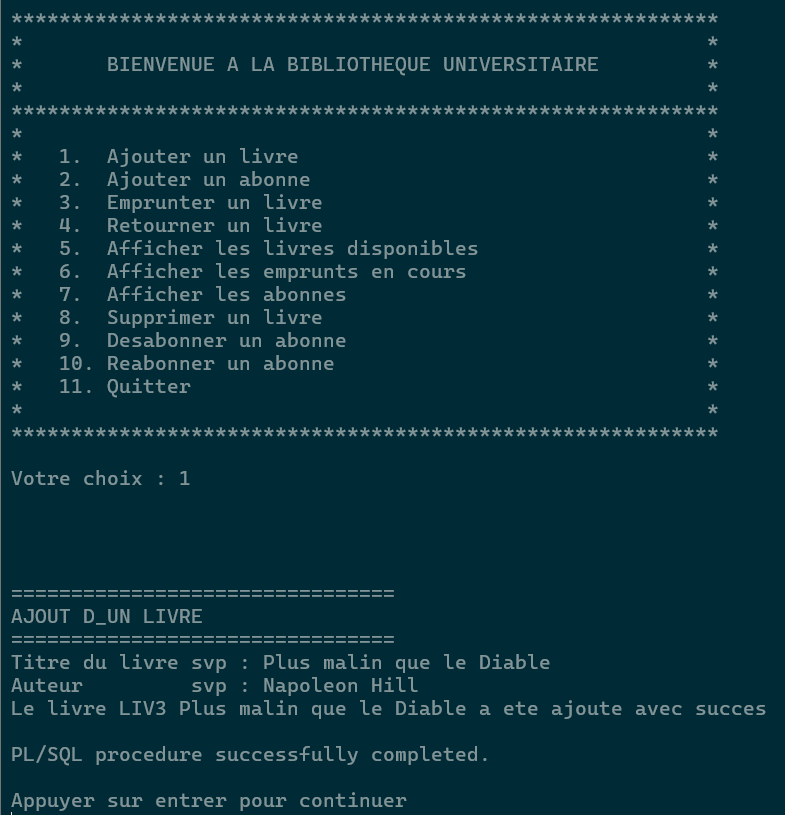
\includegraphics[width=\textwidth]{../capture_ecran/ajout_de_livre/plus_malin_que_le_diable.png}
			\caption*{Ajout du livre (LIV2) Plus Malin que le diable de Napoleon Hill}
		\end{minipage}
		
	\end{figure}
	
	\begin{figure}[H]
		\centering
		\begin{minipage}{0.6\textwidth}
			\centering
			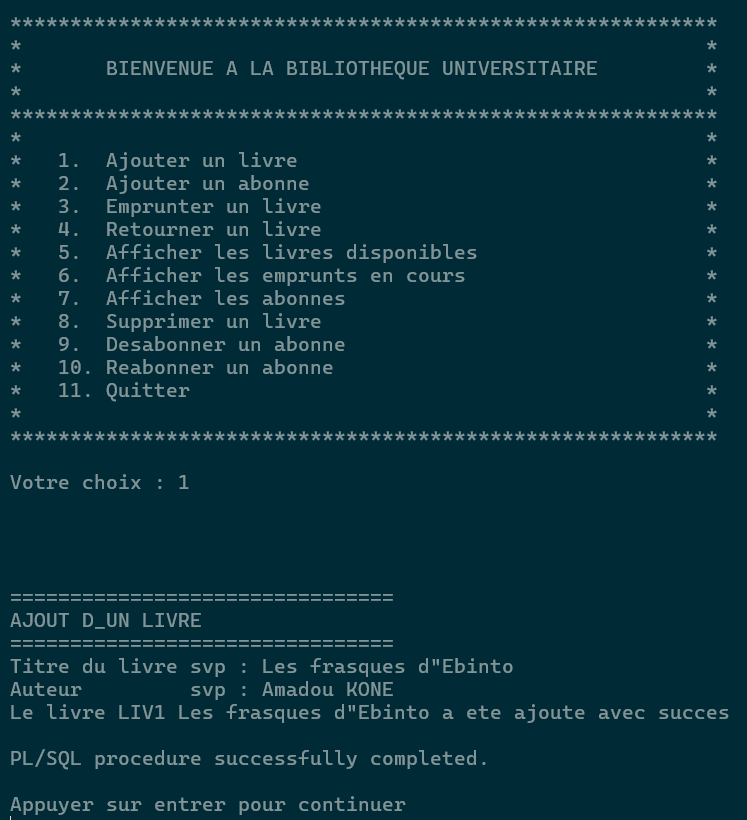
\includegraphics[width=\textwidth]{../capture_ecran/ajout_de_livre/les_frasques_d_Ebinto.png}
			\caption*{Ajout du livre (LIV3) petit Les frasques d'Ebinto de Amadou KONE}
		\end{minipage}
		\hfill
		\begin{minipage}{0.6\textwidth}
			\centering
			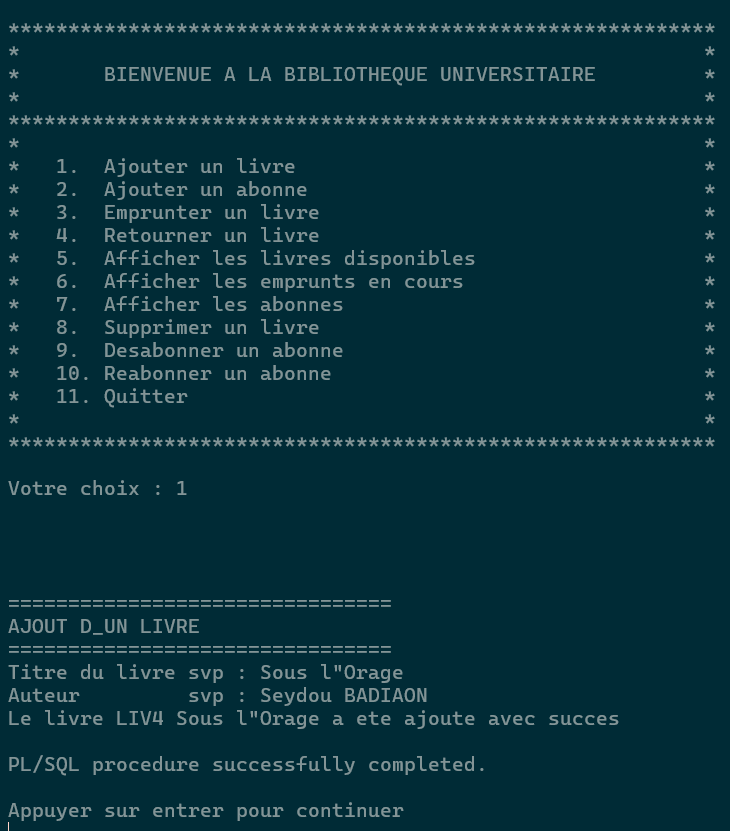
\includegraphics[width=\textwidth]{../capture_ecran/ajout_de_livre/Sous_Orage.png}
			\caption*{Ajout du livre (LIV4) Sous l'Orage de Seydou BADIAN}
		\end{minipage}
		
	\end{figure}
	
	%%%%%%%%%%%%%%%%%%%%%%%%%%%%%%%%%%%%%%%%%%%%%%%%%%%
	\section{Ajout d'abonnés}
	Ajout de 5 abonnés avec leur INE
	\begin{figure}[H]
		\centering
		\begin{minipage}{0.6\textwidth}
			\centering
			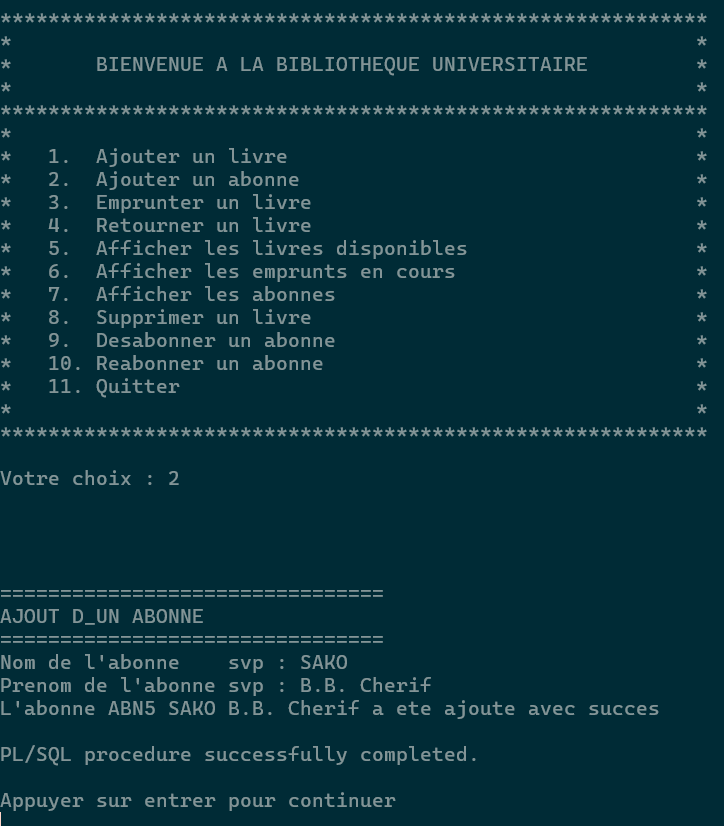
\includegraphics[width=\textwidth]{../capture_ecran/ajout_abonne/SAKO_Biton_Cherif_(N00555820231).png}
			\caption*{Ajout de l'abonné N00555820231 SAKO Biton Cherif}
		\end{minipage}
		\hfill
		\begin{minipage}{0.6\textwidth}
			\centering
			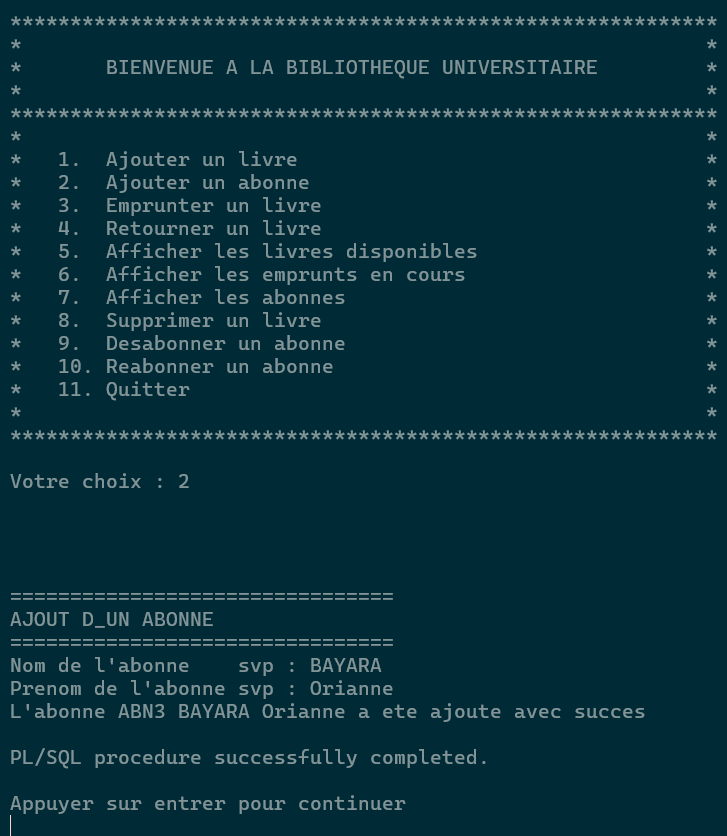
\includegraphics[width=\textwidth]{../capture_ecran/ajout_abonne/BAYARA_Oriane_(N00555820242).png}
			\caption*{Ajout de l'abonné N00555820242 BAYARA Oriane}
		\end{minipage}
		
	\end{figure}
	
	\begin{figure}[H]
		\centering
		\begin{minipage}{0.6\textwidth}
			\centering
			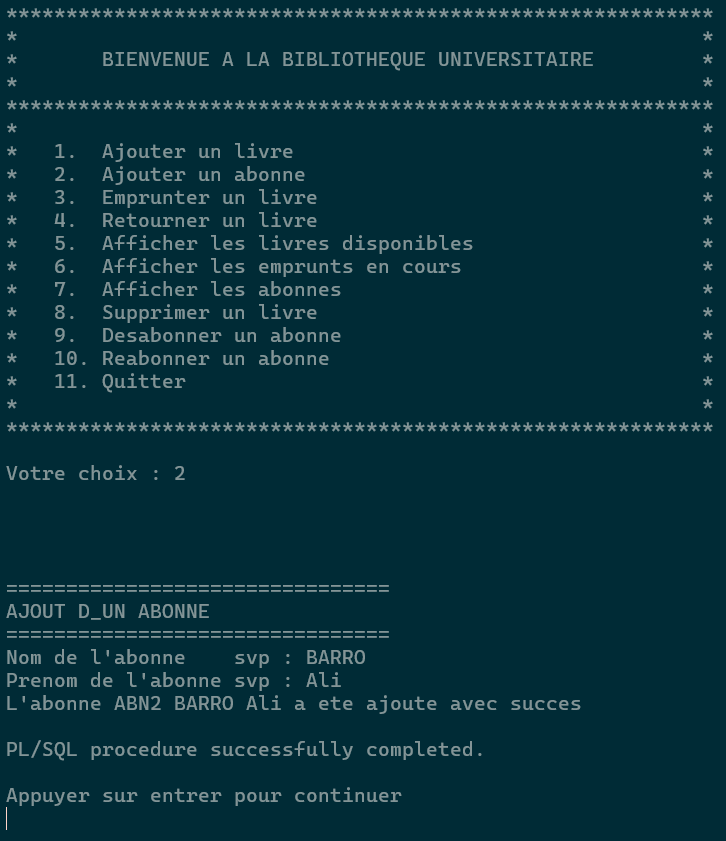
\includegraphics[width=\textwidth]{../capture_ecran/ajout_abonne/BARRO_Ali_(N00555820241).png}
			\caption*{Ajout de l'abonné N00555820241 BARRO ALI}
		\end{minipage}
		\hfill
			\begin{minipage}{0.6\textwidth}
				\centering
				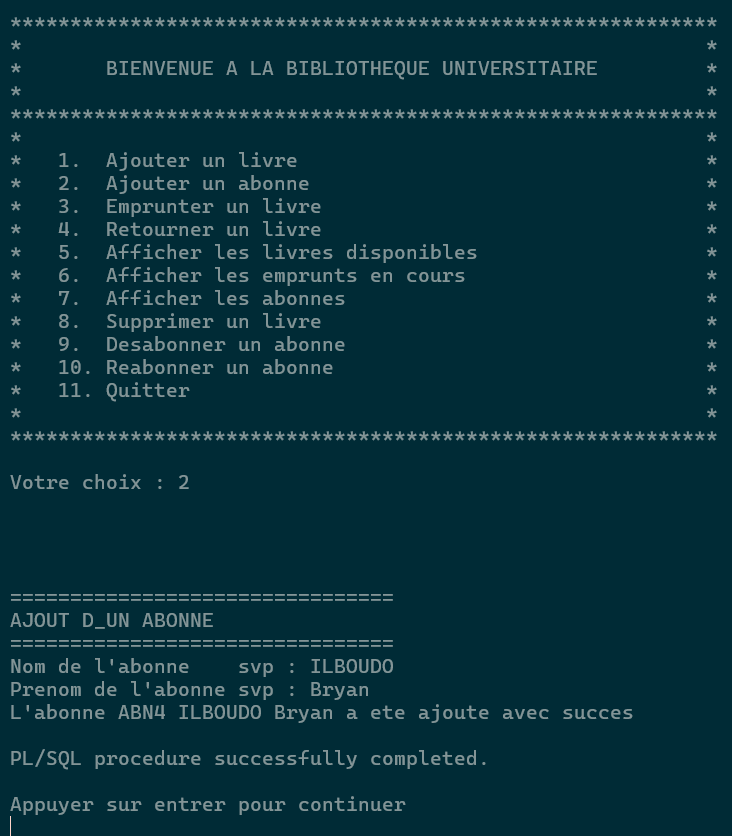
\includegraphics[width=\textwidth]{../capture_ecran/ajout_abonne/ILBOUDO_Bryand_(N00555720241).png}
				\caption*{Ajout de l'abonné N00555720241 ILBOUDO Bryand}
		\end{minipage}
		
	\end{figure}
	
	\begin{figure}[H]
		\centering
		
			\centering
			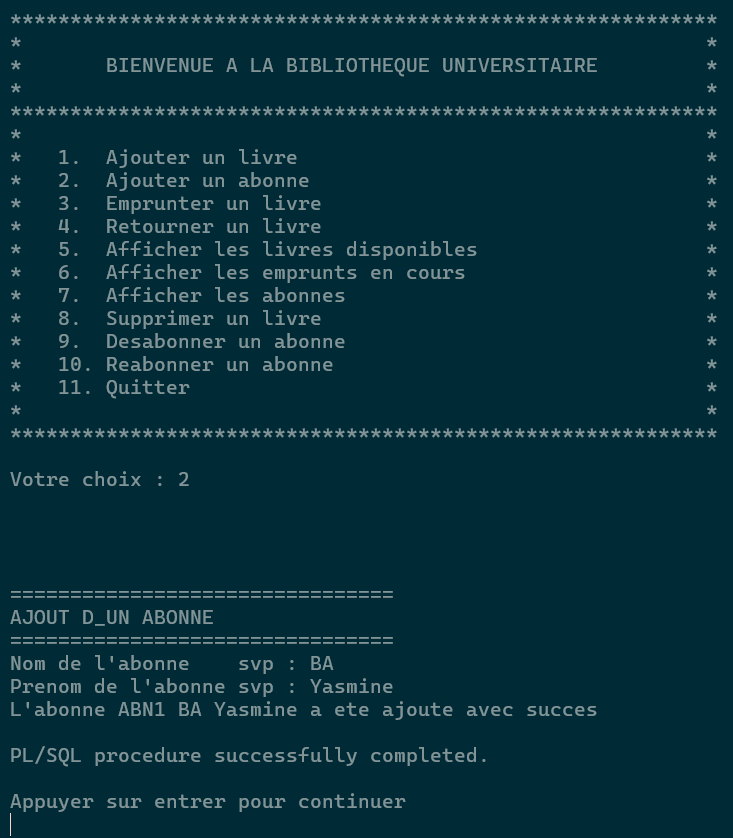
\includegraphics[width=0.6\textwidth]{../capture_ecran/ajout_abonne/BA_Yasmine_(N00555820232).png}
			\caption*{Ajout de l'abonné N00555820232 BA Yasmine}
	
	\end{figure}
	
	%%%%%%%%%%%%%%%%%%%%%%%%%%%%%%%%%%%%%%%%%%%%%%%%%%%%%%%%%%%
	
	%%%%%%%%%%%%%%%%%%%%%%%%%%%%%%%%%%%%%%%%%%%%%%%%%%%%%%%%%%%%%%%%%%
	
	
	
	\section{Emprunt d'un livre disponible par un abonné existant et actif}
	\begin{figure}[H]
		\centering
		\includegraphics[width=0.6\textwidth]{../capture_ecran/Emprunt_d_un_livre_disponible/Capture3.png}
		\caption{Emprunt d'un livre disponible par un abonné actif et existant}
	\end{figure}
	
	\section{Tentative d'emprunt d'un livre non disponible par un abonné existant et actif}
	\begin{figure}[H]
		\centering
		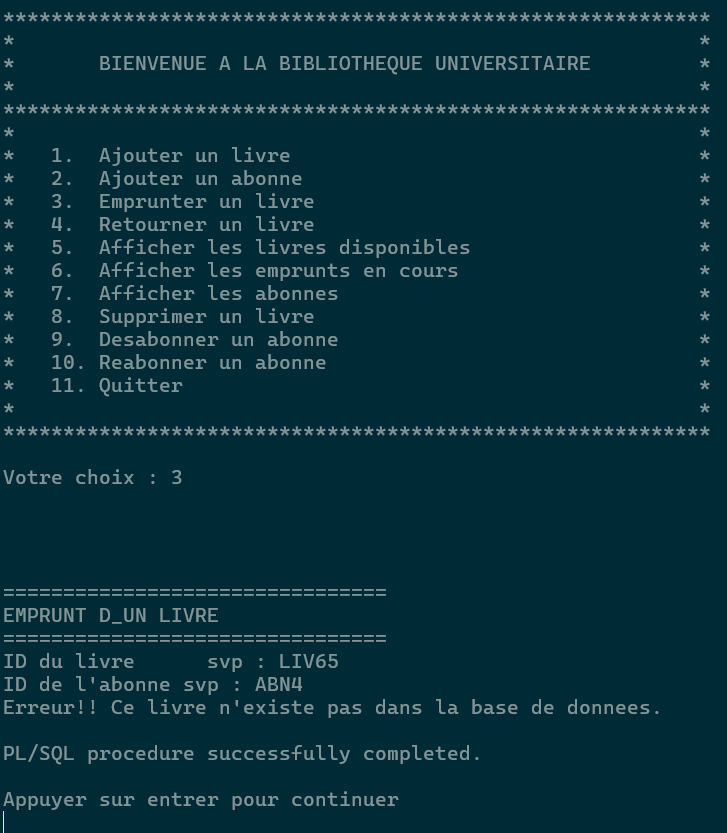
\includegraphics[width=0.6\textwidth]{../capture_ecran/Tentative_d_emprunt_d_un_livre_non_disponible/capture2.png}
		\caption{Emprunt d'un livre non disponible par un abonné actif et existant}
	\end{figure}
	
	\section{Tentative d'emprunt par un abonné existant et actif ayant déjà un emprunt en cours}
	\begin{figure}[H]
		\centering
		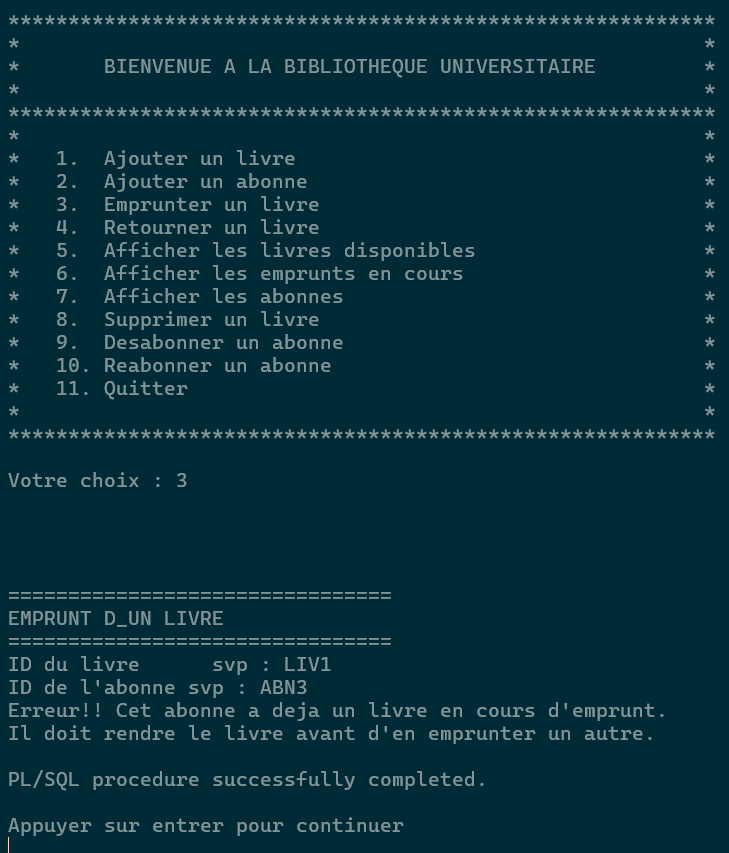
\includegraphics[width=0.6\textwidth]{../capture_ecran/emprunt_par_un_abonne_ayant_deja_un_emprunt_en_cours/capture4.png}
		\caption{Tentative d'emprunt par un abonné existant et actif ayant déjà un emprunt en cours}
	\end{figure}
	
		\section{Tentative d'emprunt d'un livre disponible par un abonné non existant }
	\begin{figure}[H]
		\centering
		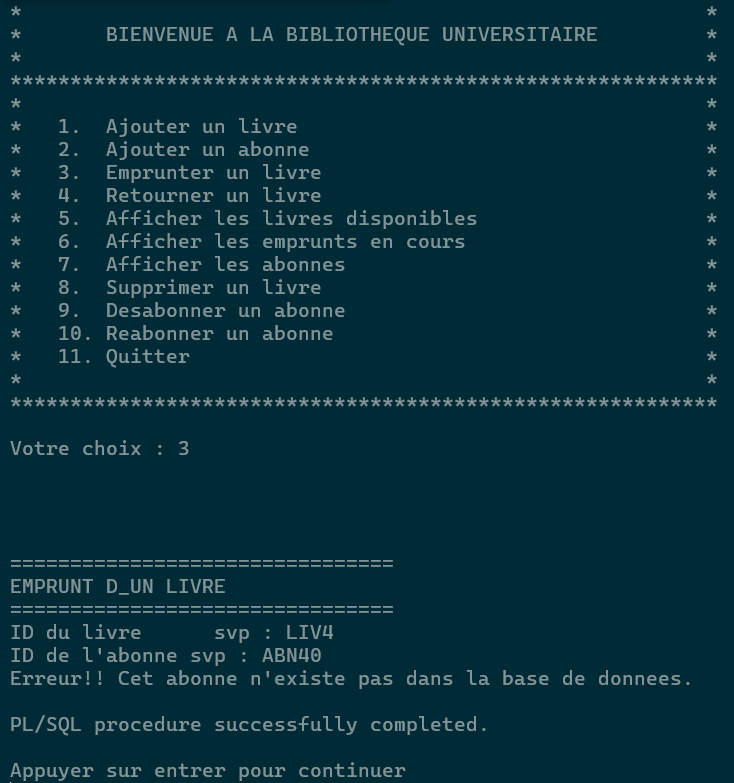
\includegraphics[width=0.6\textwidth]{../capture_ecran/emprunt_d_un_livre_disponible_par_un_abonne_non_existant/capture5.png}
		\caption{Tentative d'emprunt d'un livre disponible par un abonné non existant }
	\end{figure}
	

	\section{Retour d'un livre}
	\begin{figure}[H]
		\centering
		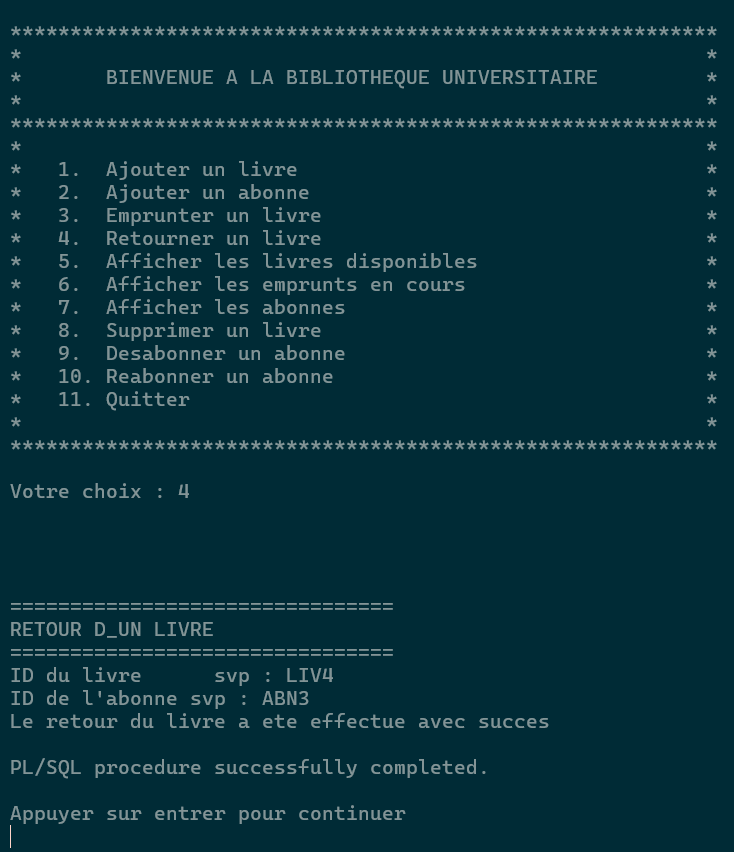
\includegraphics[width=0.6\textwidth]{../capture_ecran/retour_d_un_livre/capture6.png}
		\caption{Retour d'un livre emprunté }
	\end{figure}
	
	\section{Affichage des livres disponibles}
	\begin{figure}[H]
		\centering
		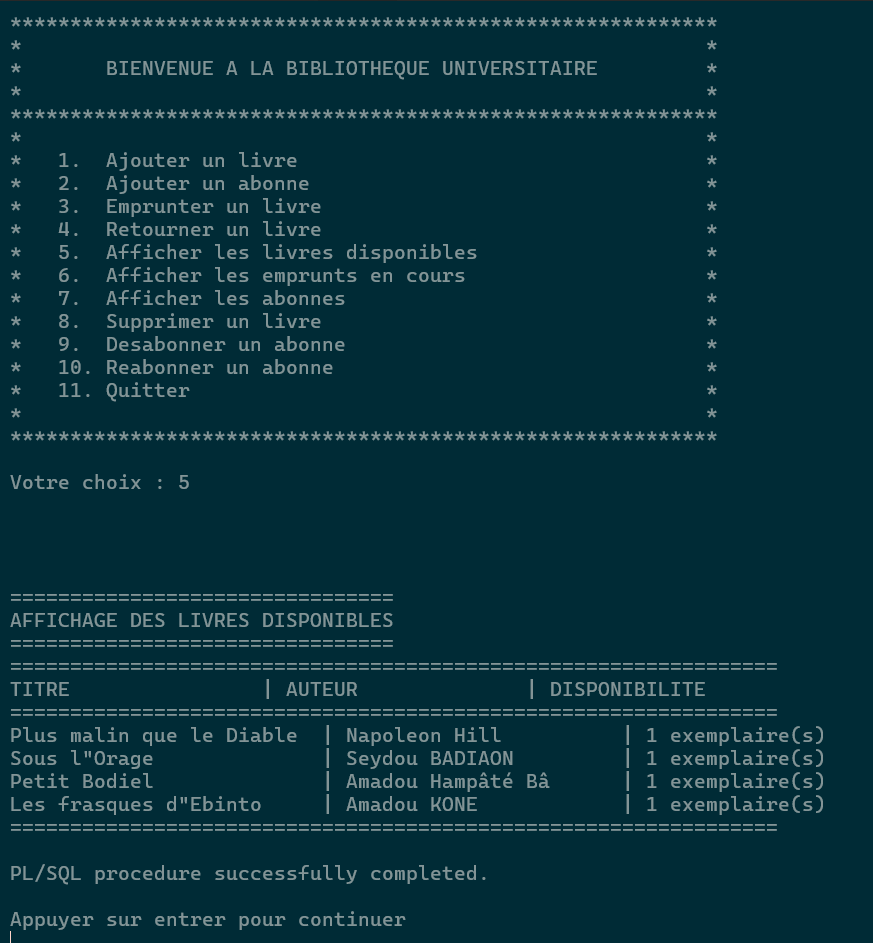
\includegraphics[width=0.6\textwidth]{../capture_ecran/Affichage_des_livres_disponibles/capture7.png}
		\caption{Affichage des livres disponibles }
	\end{figure}
	
	\section{Affichage de la liste des emprunts}
	\begin{figure}[H]
		\centering
		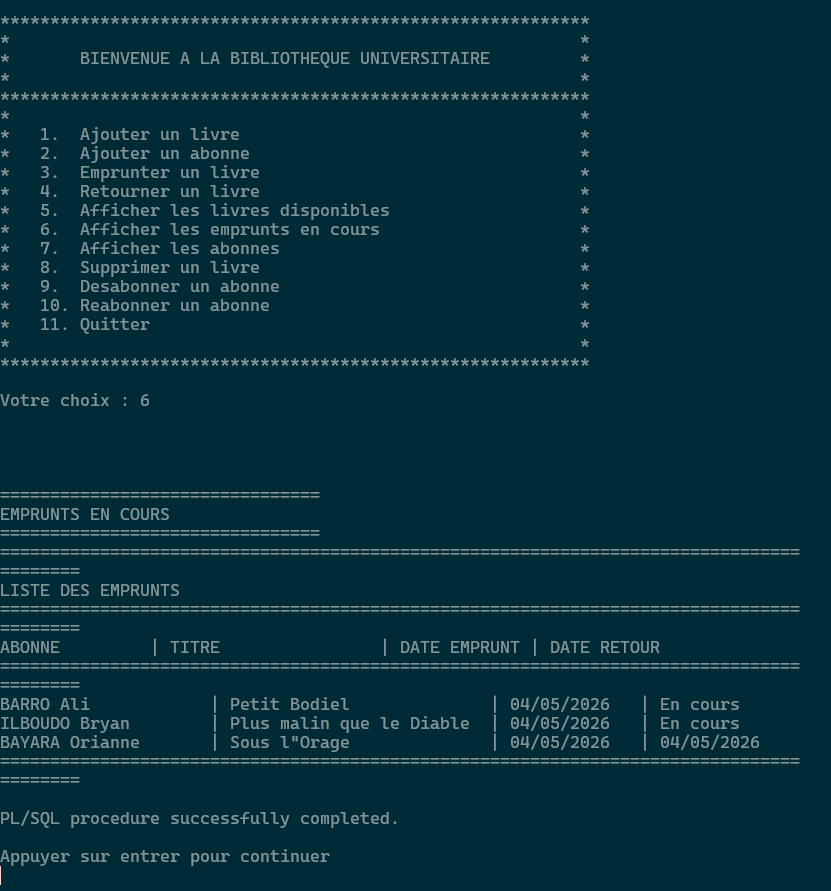
\includegraphics[width=0.6\textwidth]{../capture_ecran/Affichage_de_la_liste_des_emprunts/capture8.png}
		\caption{Affichage de la liste des emprunts }
	\end{figure}
	
	\section{Affichage de la liste des abonnés}
	\begin{figure}[H]
		\centering
		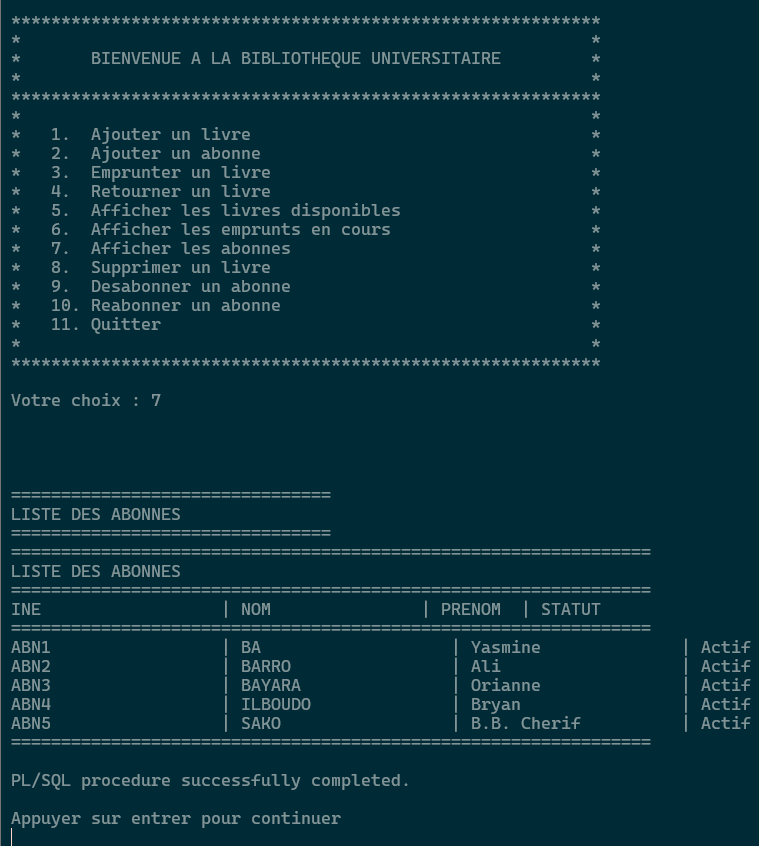
\includegraphics[width=0.6\textwidth]{../capture_ecran/Affichage_de_la_liste_des_abonnés/capture9.png}
		\caption{Affichage de la liste des abonnés}
	\end{figure}
	
	
	\section{Retrait d'un livre avec motif}
	\begin{figure}[H]
		\centering
		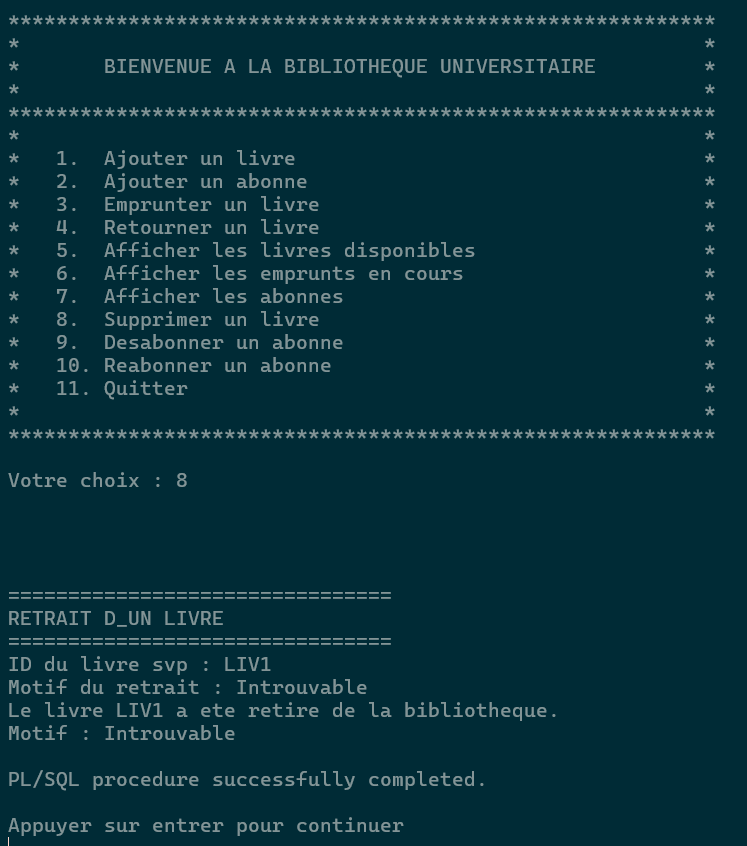
\includegraphics[width=0.6\textwidth]{../capture_ecran/Retrait_d_un_livre_dispo_non_emprunté_avec_motif/capture10.png}
		\caption{Retrait d'un livre avec motif}
	\end{figure}

	
	\section{Tentative de retrait d'un livre emprunté}
	Ici, on a effectué un emprunt du livre LIV3 par l'utilisateur N00555820241. Après cet emprunt, on tente de retirer le livre en question.
	
	\begin{figure}[H]
		\centering
		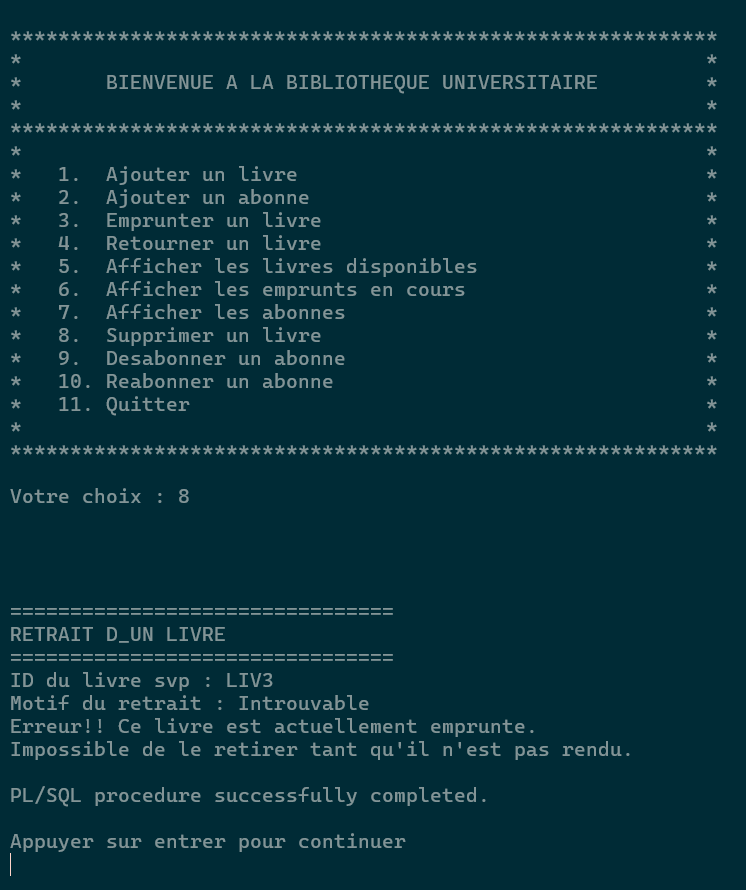
\includegraphics[width=0.6\textwidth]{../capture_ecran/Tentative_de_retrait_d_un_livre_emprunte/capture11.png}
		\caption{Tentative de retrait d'un livre emprunté}
	\end{figure}
	

	\section{Tentative de retrait d'un livre non disponible}
	\begin{figure}[H]
		\centering
		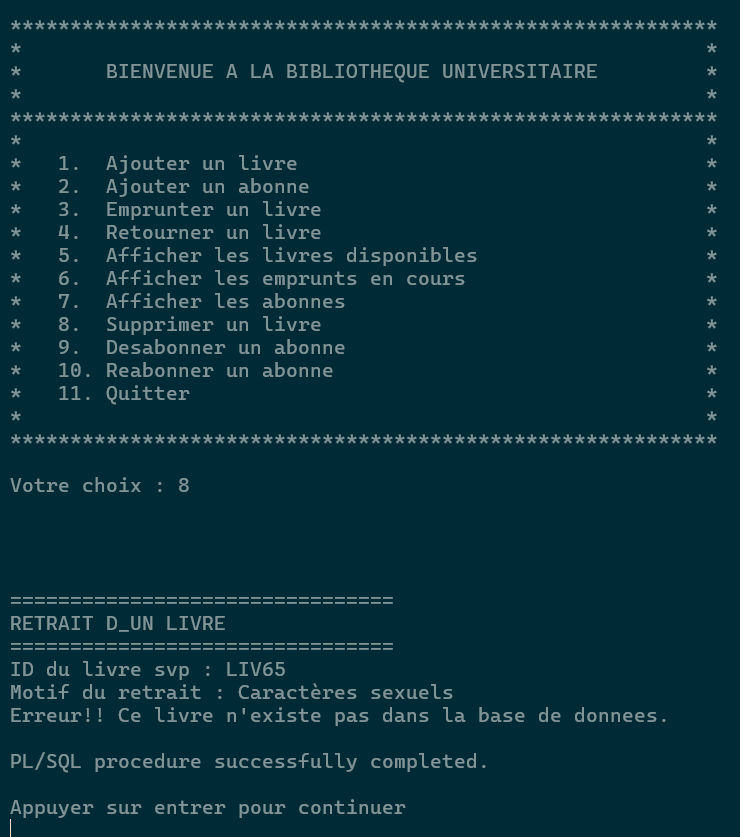
\includegraphics[width=0.6\textwidth]{../capture_ecran/Tentative_de_retrait_d_un_livre_non_disponible/capture12.png}
		\caption{Tentative de retrait d'un livre non disponible}
	\end{figure}

		\section{Désabonnement d'un abonné actif et existant avec motif}
	\begin{figure}[H]
		\centering
		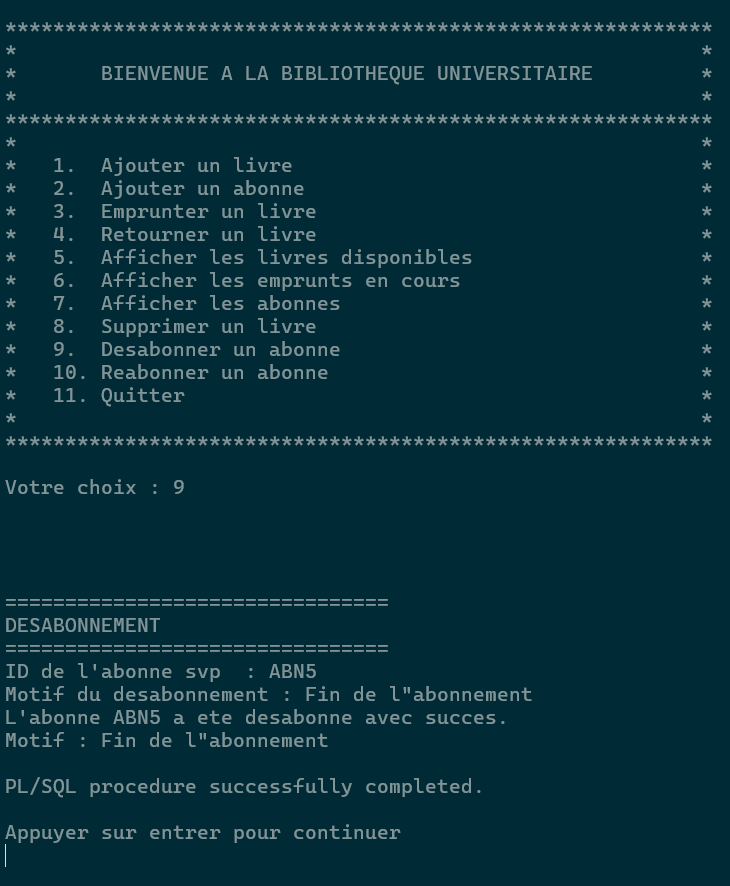
\includegraphics[width=0.6\textwidth]{../capture_ecran/Desabonnement_d_un_abonne_actif_et_existant_avec_motif/capture13.png}
		\caption{Désabonnement d'un abonné actif et existant avec motif}
	\end{figure}
	
	
		\section{Désabonnement d'un abonné inactif avec motif}
	\begin{figure}[H]
		\centering
		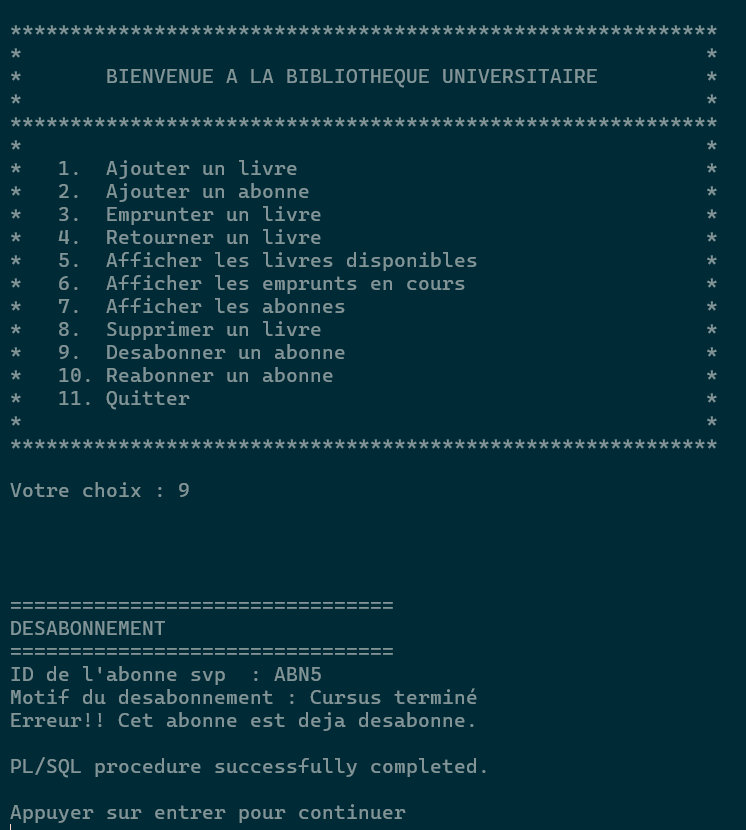
\includegraphics[width=0.6\textwidth]{../capture_ecran/Desabonnement_d_un_abonne_inactif_avec_motif/capture14.png}
		\caption{Désabonnement d'un abonné inactif avec motif}
	\end{figure}
	
		\section{ Désabonnement d'un abonné non existant avec motif}
	\begin{figure}[H]
		\centering
		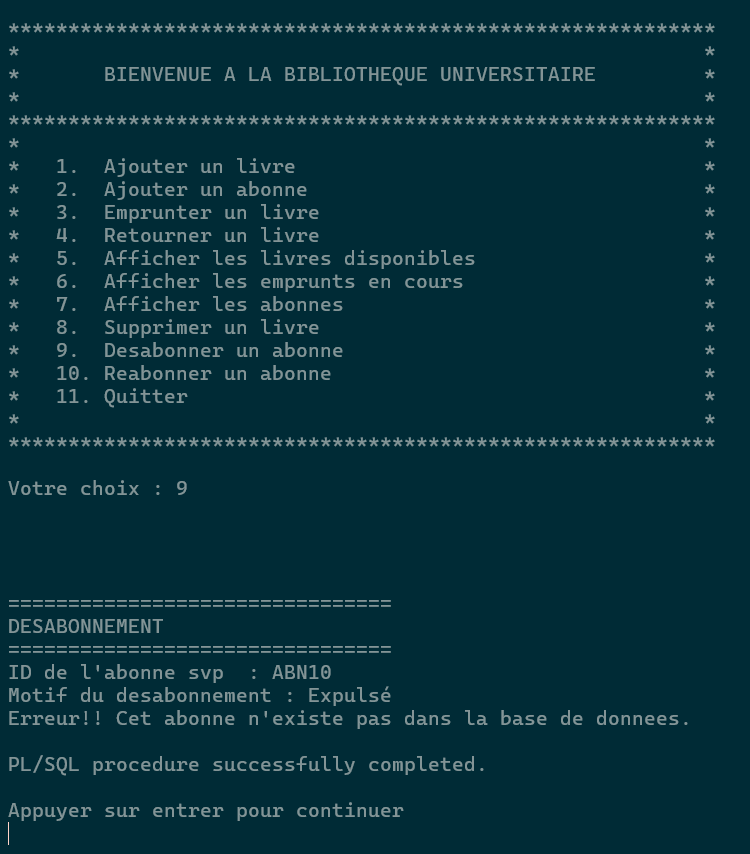
\includegraphics[width=0.6\textwidth]{../capture_ecran/Desabonnement_d_un_abonne_non_existant_avec_Motif/capture15.png}
		\caption{ Désabonnement d'un abonné non existant avec motif}
	\end{figure}

	
		\section{ Emprunt d'un livre disponible par un abonné existant et inactif}
	\begin{figure}[H]
		\centering
		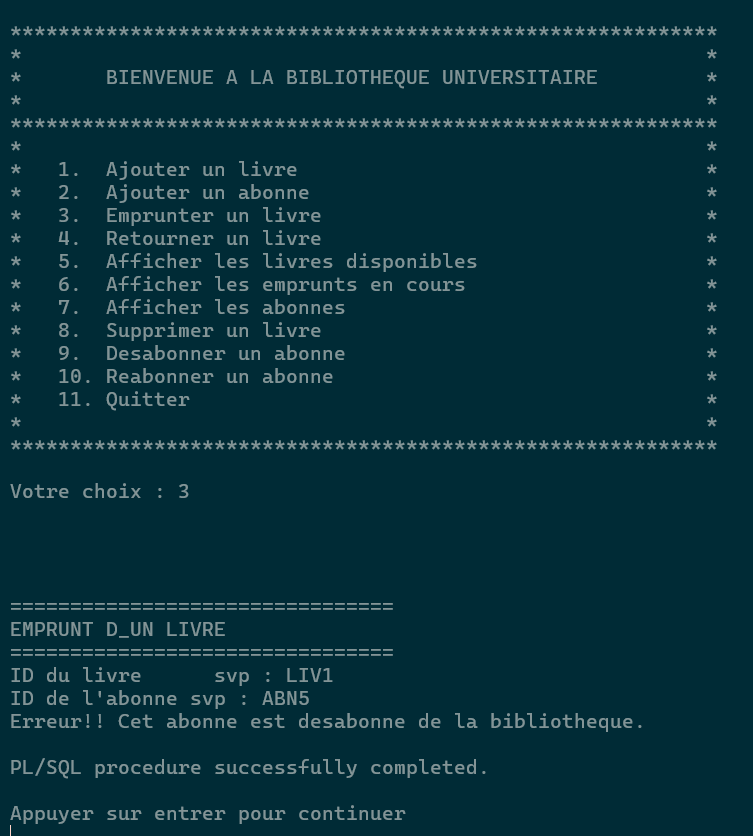
\includegraphics[width=0.6\textwidth]{../capture_ecran/Emprunt_d_un_livre_disponible_par_un_abonne_existant_et_inactif/Capture1.png}
		\caption{ Emprunt d'un livre disponible par un abonné existant et inactif}
	\end{figure}
	

		\section{ Tentative de désabonnement d'un abonné avec emprunt en cours}
	\begin{figure}[H]
		\centering
		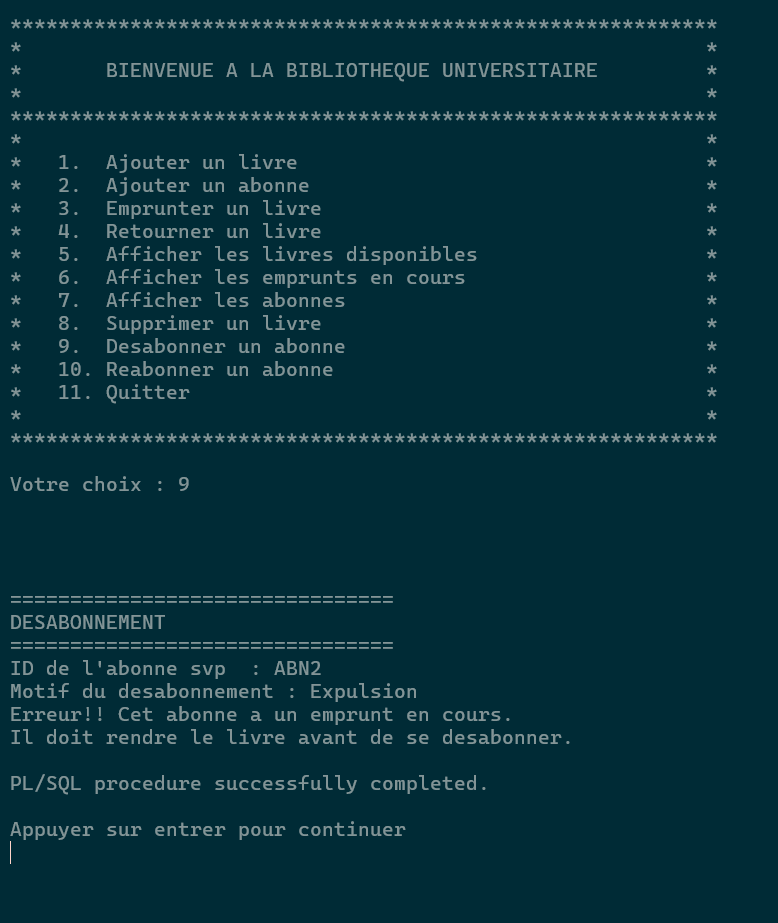
\includegraphics[width=0.6\textwidth]{../capture_ecran/Tentative_de_desabonnement_d_un_abonne_avec_emprunt_en_cours/capture16.png}
		\caption{ Tentative de désabonnement d'un abonné avec emprunt en cours}
	\end{figure}
	
		\section{Réabonnement d'un abonné inactif}
	\begin{figure}[H]
		\centering
		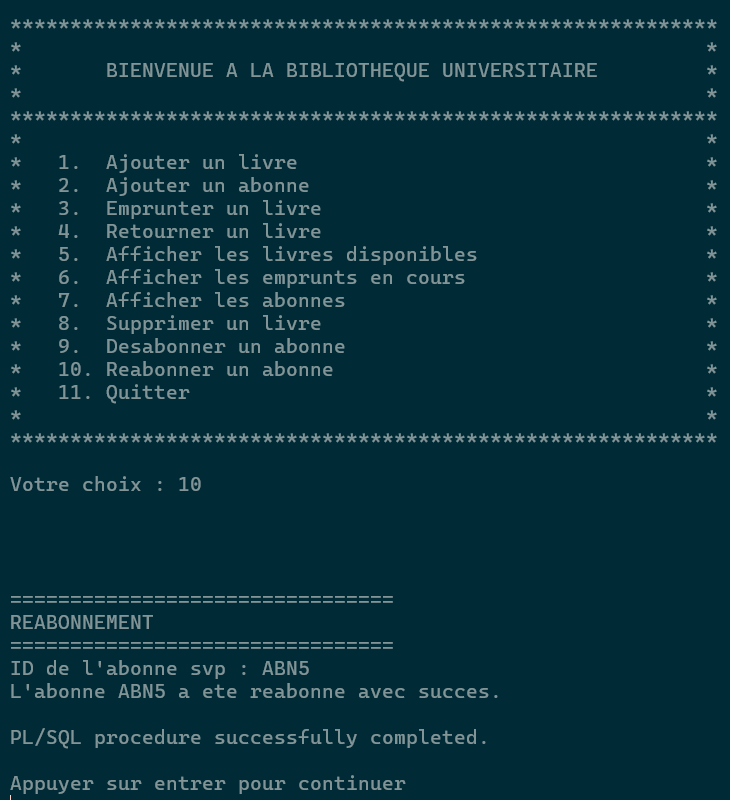
\includegraphics[width=0.6\textwidth]{../capture_ecran/Reabonnement_d_un_abonne_inactif/capture17.png}
		\caption{Réabonnement d'un abonné inactif}
	\end{figure}

	

	
	\section{Tentative de réabonnement d'un abonné déjà actif}
\begin{figure}[H]
	\centering
	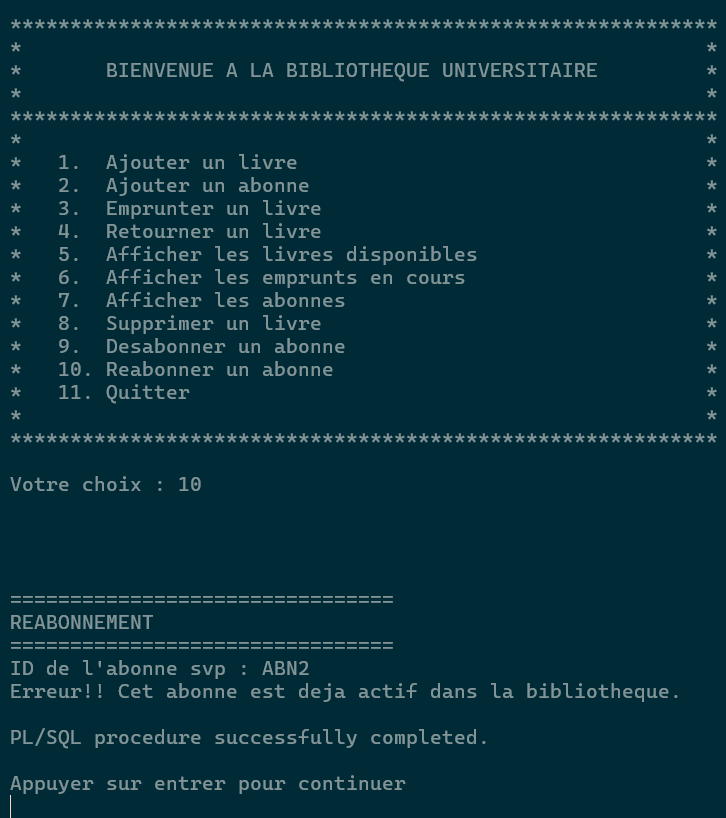
\includegraphics[width=0.6\textwidth]{../capture_ecran/Tentative_de_reabonnementd_d_un_abonne_deja_actif/capture18.png}
	\caption{Tentative de réabonnement d'un abonné déjà actif}
\end{figure}
	
	
	


% ============================================================
% CONCLUSION
% ============================================================


\chapter{Conclusion}

Ce projet nous a permis de concevoir et d'implémenter un système complet
de gestion de bibliothèque universitaire en PL/SQL. Au-delà des cinq
procédures demandées, nous avons enrichi le système avec des fonctionnalités
supplémentaires --- affichage des emprunts et abonnés, gestion des
désabonnements et réabonnements, ainsi que les retraits de livres avec
motif --- qui reflètent des besoins réels d'une bibliothèque en activité.
Le choix de la suppression logique plutôt que physique garantit la
traçabilité des données et ouvre la possibilité de réactiver un abonné
ou un livre si besoin.
L'architecture multi-fichiers adoptée pour le menu interactif offre
une séparation claire des responsabilités et rend le système facilement
extensible.
Le système développé couvre les besoins fondamentaux de gestion d'une
bibliothèque universitaire. Cependant, deux limites ont été identifiées : le
système ne distingue pas les étudiants des enseignants, alors qu'en réalité
les deux peuvent emprunter des livres dans une bibliothèque universitaire.
Dans une version améliorée, il serait pertinent d'ajouter un champ
\texttt{type} dans la table \texttt{abonne} pour différencier les deux
profils. L'identifiant resterait unique pour chacun --- l'\textbf{INE}
pour les étudiants, le \textbf{matricule} pour les enseignants --- et
les procédures existantes n'auraient pas besoin d'être modifiées en
profondeur.
De même, le système ne dispose pas de procédures de modification. Si le
bibliothécaire enregistre un livre ou un abonné avec des informations
erronées --- une faute dans le titre, un mauvais nom ou un mauvais prénom
--- il n'a aucun moyen de corriger cela sans intervenir directement en
base de données. L'ajout de procédures \texttt{modifier\_livre} et
\texttt{modifier\_abonne} constituerait donc une amélioration naturelle
et nécessaire du système.


Ce projet nous a permis de mettre en pratique les concepts fondamentaux
du PL/SQL Oracle, notamment :
\begin{itemize}
	\item La conception et la manipulation de procédures stockées
	\item L'implémentation d'un menu interactif en environnement SQL*Plus
	\item La réalisation d'opérations de gestion de données
	\item La mise en œuvre de structures de contrôle et de gestion des erreurs
\end{itemize}
\end{document}
